\subsection{I2S decoder and encoder}
The ADC and DAC use I2S to transfer the sampled audio data to the FPGA. This protocol needs to be decoded to obtain the actual data, processed and encoded again to I2S to send to the DAC. The VHDL code that has been written for this can be found in \nameref{chap:appendix-B-vhdl}. 

\subsection{I2C controller}
The DAC must be configured with I2C. To be able to do this an I2C master must be programmed in the FPGA. This I2C master initializes the DAC with default configurations. The VHDL code of the I2C master can be found in \nameref{chap:appendix-B-vhdl}. 

To initialize the DAC correctly an initializer block is made to correctly setup all the registers of the DAC using the I2C controller block. The VHDL code of this initializer block can be found in \nameref{chap:appendix-B-vhdl}. 

\subsection{Band-pass filter}
In order to successfully compute the state-space band-pass filter output, the discrete state-space coefficients are needed. The equations for the discrete coefficients are seen in equation \ref{eq:discrete-coef-Ad} and equation \ref{eq:discrete-coef-Bd}.

\begin{equation}
    Ad=e^{AT}
    \label{eq:discrete-coef-Ad}
\end{equation}

\begin{equation}
    Bd=\frac{Ad-I}{A}\cdot B
    \label{eq:discrete-coef-Bd}
\end{equation}

Because the coefficients are all matrices, doing an exponent computation is a very expensive task for an FPGA. Therefore the exponent is rewritten with the taylor series to obtain equation \ref{eq:taylor-series-Ad} and equation \ref{eq:taylor-series-Bd}. The higher the value of n in the sum for Ad and Bd the less of an effect that new value has on the sum. Therefore having the sum go from $n=0\ to\ n=10$ is more than enough for the coefficients to be almost exact. The coefficients need to be computed only at the startup of the firmware and when the parameters of the band-pass filter change. 

\begin{equation}
    Ad=\sum_{n=0}^{\infty}\frac{A^n\cdot T^n}{n!}
    \label{eq:taylor-series-Ad}
\end{equation}

\begin{equation}
    Bd=\sum_{n=1}^{\infty}\frac{A^{n-1}\cdot T^n}{n!}\cdot B
    \label{eq:taylor-series-Bd}
\end{equation}

When every sample is being loaded into the state-space band-pass filter effect, the new state variables and the output will be computed according to equation \ref{eq:state-state-equation} and equation \ref{eq:state-output-equation}. 

\begin{equation}
    \dot{x}=Ad \cdot x + Bd \cdot u
    \label{eq:state-state-equation}
\end{equation}

\begin{equation}
    y=C \cdot x + D \cdot u
    \label{eq:state-output-equation}
\end{equation}

After the computation of the state variables and the output, these data variables need to be resized to the desired size. This is necessary because when multiplying two binary numbers, the resulting numbers has the size equal to the sum of the size of the two multiplicands. The VHDL code of the state-space BPF can be found in \nameref{chap:appendix-B-vhdl}. 

\subsection{Sinewave generator}
In order to test the band-pass filter effect and the other effects, a sinewave generator is made to easily compare the input to the output of the effect. This makes the verification of the different effects very easy. The sinewave generator has an input that specifies the frequency of the generated sinewave. Because using an library that computes the sine for a certain value costs a lot of processing power, the taylor series is again used to approximate a sine. The taylor series of a sine is seen in equation \ref{eq:taylor-series-sin}. The VHDL code can be found in \nameref{chap:appendix-B-vhdl}. 

\begin{equation}
    \sin x = x - \frac{x^3}{3!} + \frac{x^5}{5!} - \frac{x^7}{7!} + \dots
    \label{eq:taylor-series-sin}
\end{equation}

\subsection{Effects}
In order to create the effects, they were first created in Matlab to test which parameters would be important and what method of making the effect would be effective. 

A paper \cite{Guitar_Effects_Processor_Using_DSP} written by Alexander J. Czubek and Gorav Raheja mentioned Simulink models for certain digital effects which needed to be implemented in this project. The Simulink models have been rewritten into Matlab code and was tested with a simple clean guitar sample to hear if the effects would work. 

The only downside is that the sample in Matlab is not processed real time. Matlab knows the samples and the order of them. So to test these effects a for-loop was written to resample the original sample so that the code could see it as a real time signal instead of a pre given file.

\subsubsection{Volume control}
The volume control is made by amplifying the input signal with a certain gain level. After the amplification the signal has to be manually clipped if out of range of the variable type. So the volume controller can be seen as an amplifier block with a saturation block. The VHDL code of this effect can be found in \nameref{chap:appendix-B-vhdl}.

\subsubsection{Distortion}
Distortion is an effect that is heard when a signal level goes beyond the saturation level. This causes the signal to go into saturation and clip (see figure \ref{fig:saturated_signal}). Normally in audio you never want distortion as this is not bearable to listen to. But for musicians, especially guitarists, the distortion effect is very popular. This is because it gives the guitar sound a lot of sustain and higher harmonics, making it very popular in rock and metal genres. 

\begin{figure}[ht]
    \centering
    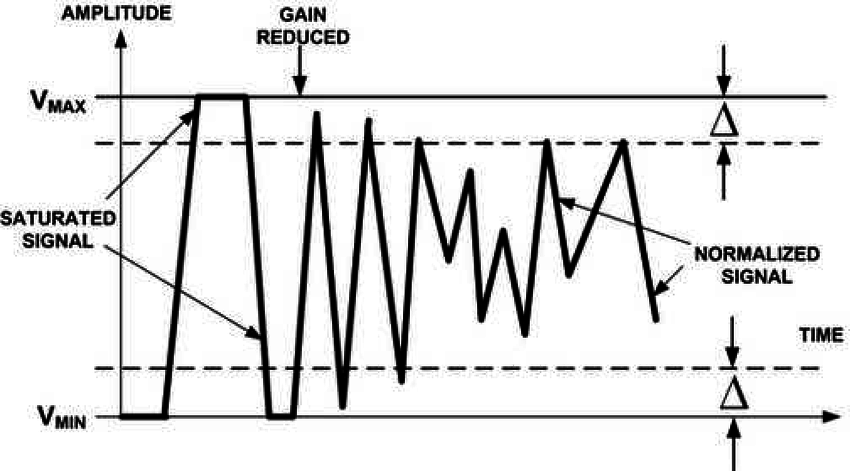
\includegraphics[width=0.5\linewidth]{Signal-Saturation-and-Gain-Control.png}
    \caption{Saturated signal}
    \label{fig:saturated_signal}
\end{figure}

So in order to make a distortion effect, the input signal needs to go into saturation. To do this, the input signal needs to be amplified a lot. So an amplifier is needed with a saturation block to clip the signal. This results in a distorted signal when you amplify the signal enough.

When the signal is amplified enough to reach the saturation point it is being distorted. But it is also very loud. Therefore it is necessary to add an attenuator after the amplifier and saturation blocks. With this attenuator the user is able to adjust the audio level of the distorted signal back to a much more bearable audio level, without changing the amount of distortion. The VHDL code of this effect can be found in \nameref{chap:appendix-B-vhdl}.

\subsubsection{Flanger}
A flanger effect delays each sample with a varying delay time adjusted by a sine wave. The delayed sample is then added to the original sample. The Simulink model of the flanger effect is seen in figure \ref{fig:flangersimulink}.

\begin{figure}[ht]
    \centering
    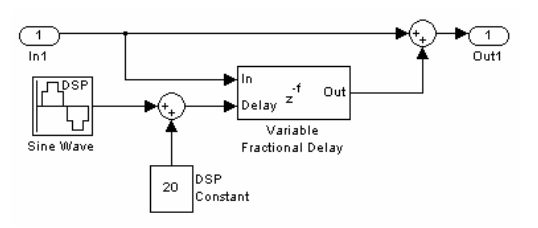
\includegraphics[width=0.5\linewidth]{flanger.png}
    \caption{Simulink model of a flanger effect}
    \label{fig:flangersimulink}
\end{figure}

\subsubsection{Chorus}
The chorus effect is created with similarities to the flanger effect. But instead of one varying delayed sample it uses four varying delay times adjusted by sine waves that have different frequencies. To a musician this sounds like there are more musicians playing the same thing. The simulink model of the chorus effect is seen in figure \ref{fig:chorussimulink}.

\begin{figure}[ht]
    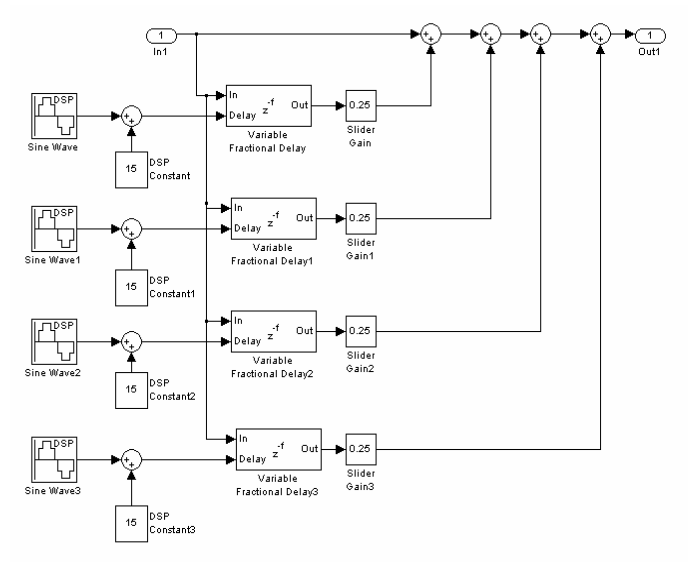
\includegraphics[width=\linewidth]{chorus.png}
    \caption{Simulink model of a chorus effect}
    \label{fig:chorussimulink}
\end{figure}

\subsubsection{Delay / echo}
The delay was the easiest of these effects to make. The delay adds a delayed sample to the original sound. The simulink model of the delay effect is seen in figure \ref{fig:delaysimulink}.

\begin{figure}[ht]
    \centering
    \includegraphics[width=0.5\linewidth]{delay.png}
    \caption{Simulink model of a delay}
    \label{fig:delaysimulink}
\end{figure}

